\documentclass[10pt]{standalone}
\usepackage{amsmath}
\usepackage{amssymb}
\usepackage{pgf,tikz}
\usepackage{mathrsfs}
\usetikzlibrary{arrows}
\pagestyle{empty}
\begin{document}
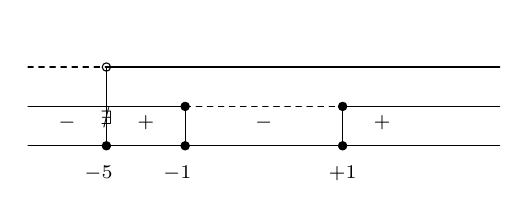
\begin{tikzpicture}[line cap=round,line join=round,>=triangle 45,x=1.0cm,y=1.0cm]
\clip(-3.,-0.5) rectangle (3.,1.5);
\draw  (-1.0,0.)-- (-1.,0.5);
\draw  (1.0,0.)-- (1.,0.5);
\draw  (-3.,0.5)-- (-1.,0.5);
\draw  (1.,0.5)-- (3.0,0.5);
\draw [dash pattern=on 2pt off 2pt] (-1.,0.5)-- (1.,0.5);
\draw  (-2.,0.)-- (-2.,1.);
\draw  (-2.,1.)-- (3.,1.);
\draw [dash pattern=on 2pt off 2pt] (-3.,1.)-- (-2.,1.);
\draw  (-3.,0.)-- (3.,0.);
\begin{scriptsize}
\draw [fill=black] (-1.,0.) circle (1.5pt);
\draw (-1.1,-0.35) node {$-1$};
\draw [fill=black] (-1.,0.5) circle (1.5pt);
\draw [fill=black] (1.,0.) circle (1.5pt);
\draw (1.0,-0.35) node {$+1$};
\draw [fill=black] (1.0,0.5) circle (1.5pt);
\draw [fill=black] (-2.0,0.) circle (1.5pt);
\draw (-2.1,-0.35) node {$-5$};
\draw (-2.5,0.3) node {$-$};
\draw (-1.5,0.3) node {$+$};
\draw (0,0.3) node {$-$};
\draw (1.5,0.3) node {$+$};
\draw(-2.,1.) circle (1.5pt);
\draw (-2.0,0.35) node {$\nexists$};
\end{scriptsize}
\end{tikzpicture}
\end{document}